\section{Binary Choice: Logit Model \& Probit Model}

Suppose $y_i \in \{0, 1\}$, the common approach is still:
\begin{align*}
    y_i &= x^{\prime} _i \beta + u_i\\
    \mathbb{E}[u_i|x_i] &= 0
\end{align*}
But, the linear regression is not attractive, because $\mathbb{E}[y_i|x_i] = \mathbb{P}[y_i=1|x_i]$ 
is bounded between 0 and 1, while the linear regression is unbounded.

We define a new regression model:
\begin{align*}
    y_i^* = x^{\prime} _i \beta + u_i \\
    u_i|x_i \sim \mathcal{N}(0, 1)
\end{align*}
and assume we have: $y_i = \mathbf{1}\{y_i^* \geq 0\}.$
If utility is positive $y_i=1$, if it is negative, $y_i=0$.

Then, we have the probability of $y_i=1$ as:
\[ 
\mathbb{P}[y_i=1]=\mathbb{P}[x_i^{\prime} \beta + u_i \geq 0] = \mathbb{P}[u_i \geq -x_i^{\prime} \beta] = 1 - \Phi(-x_i^{\prime} \beta)= \Phi(x_i^{\prime} \beta)
\]
and $\mathbb{P}[y_i=0] = 1 - \Phi(x_i^{\prime} \beta)=\Phi(-x^{\prime}_i \beta )$,
where $\Phi $ is the CDF of a standard normal RV.

Hence, $y_i$ had the PDF:
\[
p(y_i|x_i, \beta ) = \left\{\begin{matrix}
   \Phi (x_i^{\prime} \beta ) & y_i = 1\\
   \Phi (-x_i^{\prime} \beta) & y_i = 0
  \end{matrix}\right. = \Phi(x_i^{\prime} \beta )^{y_i} \Phi(-x_i^{\prime} \beta )^{1-y_i}
\]
which is the Bernoulli distribution with probability of success $\Phi(x_i^{\prime} \beta )$.

This leads to our likelihood function:
\begin{align*}
    \mathcal{L}(\beta |Y, X) &= \prod_{i=1}^{n} p(y_i|x_i, \beta )\\
    &= \prod_{i=1}^{n} \Phi(x_i^{\prime} \beta )^{y_i} \Phi(-x_i^{\prime} \beta )^{1-y_i}
\end{align*}
    
Then, we can get the log-likelihood function:
\begin{align*}
    \ell(\beta |Y, X) &= \log \mathcal{L}(\beta | Y, X)\\
    &= \sum_{i=1}^{n} \left\{y_i \log \Phi(x_i^{\prime} \beta ) + (1-y_i) \log \Phi(-x_i^{\prime} \beta )\right\}
\end{align*}
where we have the estimator defines as: $\hat{\beta} = \arg \max_{\beta} \ell(\beta|Y,X).$

Then, we can have:
\[ 
\hat{y_i} = \mathbb{E}[y_i|x_i^{\prime}, \beta ] = \Phi(x_i^{\prime} \hat{\beta}) \Rightarrow R^2 = \frac{\hat{Y}^{\prime} \hat{Y}}{Y^{\prime} Y}.
\]

The partial effect of $X$ on $Y$ is:
\begin{align*}
    \delta &= \mathbb{E}[y_i|x_i=x_2, \beta] - \mathbb{E}[y_i|x_i=x_1, \beta] \\
    &= \Phi(x_2^{\prime} \beta ) - \Phi(x_1^{\prime} \beta )\\
\end{align*}
approximately,
\[
\frac{\partial \mathbb{E}[y_i|x_i \beta]}{\partial x_i} = \frac{\partial \Phi(x_i^{\prime} \beta)}{\partial x_i} = \phi(x_i^{\prime} \beta) \beta.
\]
which is: 
\[
\Delta \mathbb{E}[y_i|x_i \beta] = \phi(x_i^{\prime} \beta ) \beta \Delta x_i.
\]

Since $\Phi(\cdot)$ is a strictly increasing function, 
the sign of $\beta_j$ reveals the sign of the partial effect of $x_{j}$,
but the size of $\beta_{j}$ is not interpretable. 
Only the relative sizes of two coefficients $\beta_k$ and $\beta_{l}$ 
have (qualitative) meaning. Nevertheless, 
we can test for the partial effect of $x_j$ being zero 
by testing $\mathcal{H}_0:\beta_j=0$, 
because the former is zero iff $\beta_j=0.$

\section{Censored Outcomes: Tobit Model}

Suppose $y_i$ is censored at 0, i.e., $y_i \geq 0$.
We can deal with this by assuming:
\begin{align*}
    y_i^* &= x_i^{\prime} \beta + u_i\\
    u_i|x_i &\sim \mathcal{N}(0, \sigma^2)\\
    y_i &= y_i^* \mathbf{1}\{y_i^* \geq 0\}
\end{align*}

In this case, the probability of observing $y_i=0$ is:
\[
\mathbb{P}[y_i=0] = \mathbb{P}[y_i^* < 0] = \mathbb{P}[x_i^{\prime} \beta + u_i < 0] = \Phi\left(-\frac{x_i^{\prime} \beta}{\sigma}\right).
\]
To get the PDF $p(y_i)$ for $y_{i}>0$, we derive the CDF:
\[ 
\mathbb{P}[y_i < y] = \mathbb{P}[y_i^* < y] = \mathbb{P}\left[\frac{u_i}{\sigma} < \frac{y-x_i^{\prime} \beta}{\sigma}\right] = \Phi\left(\frac{y - x_i^{\prime} \beta}{\sigma}\right),
\]
which gives that
\[
p(y) = \frac{\partial \mathbb{P}[y_i < y]}{\partial y} = \frac{1}{\sigma} \phi\left(\frac{y - x_i^{\prime} \beta}{\sigma}\right)
\]
for $y>0$.

Hence, the PDF observations $y_i$ is:
\[
p(y_i|x_i, \beta, \sigma) = \left\{\begin{matrix}
    \Phi\left(-\frac{x_i^{\prime} \beta}{\sigma}\right) & y_i = 0\\
    \frac{1}{\sigma} \phi\left(\frac{y_i - x_i^{\prime} \beta}{\sigma}\right) & y_i > 0
\end{matrix}\right.
\]

Then, we can get the likelihood function:
\begin{align*}
    \mathcal{L}(\beta, \sigma |Y, X) &= \prod_{i=1}^{n} p(y_i|x_i, \beta, \sigma)\\
    &= \prod_{i=1}^{n} \left\{\Phi\left(-\frac{x_i^{\prime} \beta}{\sigma}\right)\right\}^{1\{y_i=0\}} \left\{\frac{1}{\sigma} \phi\left(\frac{y_i - x_i^{\prime} \beta}{\sigma}\right)\right\}^{1\{y_i>0\}}
\end{align*}
    
Then, we can get the log-likelihood function:
\begin{align*}
    \ell(\beta, \sigma |Y, X) &= \log \mathcal{L}(\beta, \sigma | Y, X)\\
    &= \sum_{i=1}^{n} \left\{ \mathbf{1}\{y_i=0\} \log \Phi\left(-\frac{x_i^{\prime} \beta}{\sigma}\right) + \mathbf{1}\{y_i>0\} \log \left(\frac{1}{\sigma} \phi\left(\frac{y_i - x_i^{\prime} \beta}{\sigma}\right)\right)\right\}
\end{align*}
Let $\mathcal{G} = \{i, y_i = 0\}$, we can wirte the log-likelihood function as:
\begin{align*}
    \ell(\beta, \sigma |Y, X) &= \sum_{i \in \mathcal{G}} \left\{ \log \Phi\left(-\frac{x_i^{\prime} \beta}{\sigma}\right)\right\} + \sum_{i \notin \mathcal{G}} \left\{\log \left(\frac{1}{\sigma} \phi\left(\frac{y_i - x_i^{\prime} \beta}{\sigma}\right)\right)\right\}
\end{align*}

Our estimator is defined as: 
\[\hat{\theta}_{ML} = (\hat{\beta}_{ML} , \hat{\sigma}_{ML}^2 ) = \arg \max_{\theta = (\beta, \sigma)} \ell(\theta|Y, X).
\]

To compute partial effects, 
we need to derive the (conditional) expectation $\mathbb{E}[y_i|x_i].$ 
Using the result that for $Z\sim N(0,1)$, 
$\mathbb{E}[Z|Z>-c]=\phi(c)/\Phi(c)$ (\textcolor{red}{inverse Mills ratio}), we get
\[
\mathbb{E}[y_i|y_i>0]=\mathbb{E}[x_i'\beta+u_i|u_i>-x_i'\beta]=x_i'\beta+\sigma\phi\left(\frac{x_i'\beta}{\sigma}\right)/\Phi\left(\frac{x_i'\beta}{\sigma}\right).
\]

\begin{note}[Inverse Mills Ratio]
    \

    The inverse Mills ratio is the ratio of the 
    probability density function to the complementary 
    cumulative distribution function of a distribution. 
    Its use is often motivated by the following property 
    of the truncated normal distribution. 
    If $X$ is a random variable having a normal distribution 
    with mean $\mu$ and variance $\sigma^2$, then
    \begin{align*}
        \mathbb{E}[\:X\mid X>\alpha\:]&=\mu+\sigma\frac{\phi\Big(\frac{\alpha-\mu}\sigma\Big)}{1-\Phi\Big(\frac{\alpha-\mu}\sigma\Big)},\\
        \mathbb{E}[\:X\mid X<\alpha\:]&=\mu-\sigma\frac{\phi\Big(\frac{\alpha-\mu}\sigma\Big)}{\Phi\Big(\frac{\alpha-\mu}\sigma\Big)}
    \end{align*}
    where $\alpha$ is a constant, 
    $\phi$ denotes the standard normal density function, 
    and $\Phi$ is the standard normal cumulative distribution function.

    The two fractions are the inverse Mills ratios.
\end{note}

Then, we obtain
\begin{align*}
    \mathbb{E}[y_i] &= \mathbb{E}[y_i|y_i \geq 0] \mathbb{P}[y_i \geq 0] \\
    &= \mathbb{E}[y_i|y_i = 0]\mathbb{P}[y_i = 0] + \mathbb{E}[y_i|y_i > 0]\mathbb{P}[y_i > 0]\\
    &= \mathbb{E}[y_i|y_i > 0](1-\mathbb{P}[y_i = 0])\\
    &= \mathbb{E}[y_i^*|y_i^*>0]\left(1-\Phi\left(\frac{-x_i^{\prime} \beta}{\sigma}\right)\right)\\
    &= \mathbb{E}[x_i^{\prime} \beta + u_i|u_i +x_i^{\prime} \beta>0]\left(1-\Phi\left(\frac{-x_i^{\prime} \beta}{\sigma}\right)\right)\\
    &= \mathbb{E}[x_i^{\prime} \beta + u_i|u_i > -x_i^{\prime} \beta]\left(1-\Phi\left(\frac{-x_i^{\prime} \beta}{\sigma}\right)\right)\\
    &= x_i^{\prime} \beta + \sigma \frac{\phi(x_i^{\prime} \beta/\sigma)}{\Phi(x_i^{\prime} \beta/\sigma)}\left(1-\Phi\left(\frac{-x_i^{\prime} \beta}{\sigma}\right)\right)\\
    &= \Phi\left(\frac{x_i^{\prime} \beta}{\sigma}\right)\left(x_i^{\prime} \beta +\sigma \frac{\phi\left(\frac{x_i^{\prime} \beta}{\sigma}\right)}{\Phi\left(\frac{x_i^{\prime} \beta}{\sigma}\right)}\right)\\
    &= \Phi \left(\frac{x_i^{\prime} \beta}{\sigma}\right) x_i^{\prime} \beta +\sigma \phi\left(\frac{x_i^{\prime} \beta}{\sigma}\right).
\end{align*}

\section{Marginal Effects of Nonlinear Models(Probit, Logit, Tobit. etc.)}

\begin{note}
    \ 
    
    \textcolor{red}{$\beta_{MLE}$ is not the marginal effect of $y_i$, but it can be regarded as the marginal effect of potential variable $y_i^*$.}
\end{note}

\underline{Expectation and marginal effect of $y_i^*$}
\begin{align*}
    \mathbb{E}[y_i^*|x_i] &= x_i^{\prime} \beta\\
    \frac{\partial \mathbb{E}[y_i^*|x_i]}{\partial x_{ij}} &= \beta_j
\end{align*}

\underline{Truncated Models}
\begin{align*}
    \mathbb{E}[y_i \mid y_i>0, x_i] &= x_i^{\prime} \beta + \mathbb{E}[u_i \mid u_i > -x_i^{\prime} \beta] \\
    &= x_i^{\prime} \beta +  \sigma \lambda\left(\frac{x_i^{\prime} \beta}{\sigma}\right)
\end{align*}
where $\lambda = \frac{\phi(x_i^{\prime} \beta/\sigma)}{\Phi(x_i^{\prime} \beta/\sigma)}$ is the inverse Mills ratio.

\begin{align*}
    \frac{\partial \mathbb{E}[y_i \mid y_i>0, x_i]}{\partial  x_j} &= \beta_j + \sigma \frac{\partial \lambda}{\partial x_j} \\
    &= \beta_j + \sigma \frac{\partial \lambda}{\partial c} \frac{\partial c}{\partial x_j} \\
    &= \beta_j + \frac{\partial \lambda}{\partial c} \beta_j \\
    &= \beta_j \left\{ 1 - \lambda \left(\frac{x_i^{\prime} \beta}{\sigma}\right) \left[ \frac{x_i^{\prime} \beta}{\sigma} + \lambda \left(\frac{x_i^{\prime} \beta}{\sigma}\right) \right] \right\}
\end{align*}
So, we could tell that the effect of $x_j$ on $y_i$ is not only affected by $\beta_j$, but also affected by $\frac{x_i^{\prime} \beta}{\sigma}$.

\underline{Censored Models}
\begin{align*}
    \mathbb{E}[y_i \mid x_i] &= \mathbb{P}[y_i>0 \mid x_i] \cdot \mathbb{E}[y_i \mid y_i>0, x_i] \\
    &= \Phi\left(\frac{x_i^{\prime} \beta}{\sigma}\right) \mathbb{E}[y_i \mid y_i>0, x_i] \\
    \frac{\partial \mathbb{E}[y_i \mid x_i]}{\partial x_j} &= \frac{\partial \mathbb{P}[y_i>0 \mid x_i]}{x_j} \mathbb{E}[y_i \mid y_i>0, x_i] + \mathbb{P}[y_i>0 \mid x_i] \frac{\partial \mathbb{E}[y_i \mid y_i>0, x_i]}{x_j} \\
    &= \beta_j \Phi\left(\frac{x_i^{\prime} \beta}{\sigma}\right)
\end{align*}

\begin{table}[H]
    \centering
    \begin{tabular}{|c|c|}
    \hline
    \textbf{Derivative Function} & \textbf{Gradient} \\ \hline
    Optimal Response $y^*$       & $\frac{\partial E(y^* \mid x)}{\partial x_j} = \beta_j$ \\ \hline
    Positive Response $y$ (censored at 0) & $\frac{\partial E(y \mid y>0, X)}{\partial x_j} = \beta_j \{1 - \lambda(c)[c + \lambda(c)]\}$ \\ \hline
    Non-zero Response $y$ (censored at 0) & $\frac{\partial E(y \mid x)}{\partial x_j} = \beta_j \Phi(c)$ \\ \hline
    \end{tabular}
    \caption{Note: $c = \frac{x^{\prime}  \beta}{\sigma}$}
\end{table}

\pagebreak
\section{Censored, truncated or sample-selected data \protect\footnote{This part is borrowed from Xiang Ao, March 24, 2009, \textit{An Introduction to censored, truncated or sample-selected data}, Harvard Business School.}}
\begin{table}[H]
    \centering
    \caption{Comparison of censored, truncated, and sample-selected cases. (borrowed from Richard Breen)}
    \begin{tabular}{|>{\raggedright\arraybackslash}m{2cm}|>{\raggedright\arraybackslash}m{4cm}|>{\raggedright\arraybackslash}m{4cm}|>{\raggedright\arraybackslash}m{4cm}|}
    \hline
    \textbf{Sample} & \textbf{$Y$ Variable} & \textbf{$X$ Variable} & \textbf{Example} \\ \hline
    Censored & $y$ is known exactly only if some criterion defined in terms of $y$ is met. & $x$ variables are observed for the entire sample, regardless of whether $y$ is observed exactly & Determinants of income; income is measured exactly only if it above the poverty line. All other incomes are reported at the poverty line \\ \hline
    Selected & $y$ is observed only if a criteria defined in terms of some other random variable (Z) is met. & $x$ and $w$ (the determinants of whether $Z$ = 1) are observed for the entire sample, regardless of whether $y$ is observed & Survey data with item or unit non-response \\ \hline
    Truncated & $y$ is known only if some criterion defined in terms of $y$ is met. & $x$ variables are observed only if $y$ is observed. & Donations to political campaigns \\ \hline
    \end{tabular}
\end{table}

\begin{definition}[Truncated]
    A sample is truncated if some observations are systematically excluded from
the sample.
\end{definition}

\begin{eg}
    \

    Suppose we are interested in relationship between people's income($y$) and education($x$). 
    If we have observations of both $y$ and $x$ only for people whose income is above \$20,000 per year,
    then we have a truncated sample. 
\end{eg}

\begin{definition}[Censored]
    \

    A sample is censored if no observations have been systematically excluded but some of information contained in them has been suppressed.
\end{definition}

\begin{eg}
    \

    If we don't observe people's income ($y$) and education($x$)
    with income lower than \$20,000 per year, then we have a truncated sample.
    If we have observations of $x$ for people whose income above AND below that limit,
    but no information on exactly how much their income is for those whose income below the limit 
    (only thing we know is that it's lower than \$20,000 per year), then we have a censored sample.
\end{eg}

\includepdf[addtotoc={1,section,1,title in toc,cc},pages=3-7,offset=0cm 0cm]{lectures/censored_selected_truncated.pdf}